\section{Particle Dark Matter \Contact{Haibo}}
\Contributors{Haibo, Alex, Francis-Yan}
\label{sec:particles}

%\footnote{WIMPs and axions are not truly ``collisionless" because they require a coupling with other particles during their birth epoch in the early universe.  However, their interactions are so small that they are effectively collisionless particles for cosmology applications after that epoch.  Hence, WIMPs and axions are often considered to be the canonical examples of particle models for the CDM paradigm even though they are technically not completely collisionless.\AHGP{I added this.  Not sure this is the best place for it, but it would be good if this idea went somewhere.}}  

The standard \LCDM cosmological model assumes that dark matter is fully nonrelativistic and interacts purely via gravitational interactions during the process of structure formation. However, a significant dark matter thermal velocity dispersion or the presence of large non-gravitational interactions in the dark sector, such as dark matter self-interactions, couplings to other dark sector particles, or couplings to Standard Model particles, can alter the distribution of dark matter in ways that are observable with LSST. Here we focus on three minimal but representive extensions to CDM -- warm dark matter (WDM), self-interacting dark matter (SIDM), and baryon-scattering dark matter (BSDM) --  to demonstrate how measurements of the distribution of dark matter can be used to constrain micro-physical particle properties of dark matter. We largely leave in-depth discussion of the particle physics responsible for producing these models to the literature; however, we do attempt to connect astrophysical observables to specific terms in the interaction Lagrangian for these models.



%The observable impact of specific dark matter particle candidates has been examined extensively in the literature \citep[\eg,][]{2012MNRAS.423.3740V,2013MNRAS.431L..20Z,2013MNRAS.430..105P,Rocha:2012jg,Lovell:2013ola,Buckley:2014ab,1512.05344, 1512.05349,Bose:2016irl,Mocz:2017wlg}, and  we do not attempt to present a comprehensive overview of the landscape of dark matter models.Rather, we focus on three minimal extensions to CDM -- warm dark matter (WDM), self-interacting dark matter (SIDM), and baryon-scattering dark matter (BSDM) --  to demonstrate how measurements of the distribution of dark matter can be used to constrain microphysical particle properties of dark matter.We largely leave in-depth discussion of the particle physics responsible for producing these models to the literature; however, we do attempt to connect astrophysical observables to specific terms in the interaction Lagrangian for these models.

\subsection{Warm Dark Matter (WDM)}
\label{sec:wdm}

%The warm dark matter candidate a long free-streaming length, resulting in a cutoff on halo abundance for low-mass halos. In the warm dark matter theory, dark matter typically has a light mass around few keV such that it decouples from the thermal bath late and lead to a long free-streaming length. Typical warm dark matter candidates include sterile neutrinos. In warm dark matter, structure formation of the universe occurs bottom-up above the free-streaming scale, while top-down for scale below the free-streaming scale. The measurements of the Lyman-alpha forest put lower bounds on the mass of warm dark matter produced thermally 3.5 (5.3) keV [], corresponding to the minimal halo mass $10^9\textup{--}10^{10}M_\odot$.

In the standard thermal dark matter paradigm, primordial inhomogeneities in the matter density field are washed out by collisional damping and free streaming of particle dark matter \citep{Hofmann:2001,Green:2003un, Bertschinger:2006nq, Loeb:2005pm}.  
For a canonical 100-GeV thermal relic dark matter particle \citep[\eg, the WIMP;][]{Jungman:1995df}, these processes erase cosmological perturbations with $M \leq 10^{-6} \Msun$ \citep[i.e., Earth mass;][]{Green:2003un}. 
Lighter particles continue to free stream until later times, thus suppressing the formation of structure at higher mass scales (\eg, structure formation occurs bottom-up above the free-streaming scale and top-down for scales below the free-streaming scale). Because these particles are created while they are semi-relativistic, they are conventionally referred to as warm dark matter (WDM) \citep{Bond:1983hb,Bode:2000gq,Dalcanton:2000hn}. 

One well-motivated WDM candidate is a sterile neutrino $\nu_{\rm s}$ with a mass in the keV range \citep[\eg][]{Abazajian:2017tcc,Adhikari:2017}. The most relevant Lagrangian term in this case is simply the Majorana mass term
\begin{equation}
    \mathcal{L} \supset -\frac{1}{2}M_{\rm s}\bar{\nu}_{\rm s} \nu_{\rm s}.
\end{equation}
Interestingly, such a sterile neutrino can typically mix with active Standard Model neutrinos \citep[see \eg][]{Asaka:2005an}, allowing the former to decay and leading to a potentially observable X-ray signal \citep{Abazajian:2001vt}. A possible hint of such a signal has been found in deep X-ray data in the form of a narrow 3.5 keV line \citep{Boyarsky:2014, Bulbul:2014, Boyarsky:2015, Iakubovskyi:2015}, which has prompted renewed interest in understanding structure formation in WDM cosmologies \citep[see \eg][]{Lovell:2013ola,Bose:2016irl,Bozek:2018ekc}. Generally speaking, both the sterile neutrino mass and its thermal history play an important role in determining the small-scale dark matter distribution within any given particle model. For instance, at a fixed particle mass, a species created in the early Universe with a velocity distribution that is skewed towards low-momentum particles \citep[\eg][]{Shi:1998km,Venumadhav:2015pla} will display less free-streaming damping of cosmological structure than a species with a thermal (Fermi-Dirac) distribution. To avoid ambiguity, it is customary to quote WDM constraints simply in terms of a particle mass $m_{\rm WDM}$, assuming that the DM followed a thermal distribution at early times.

The free-streaming scale can be approximated by the (comoving) size of the horizon when the WDM particles become nonrelativistic. 
%The comoving horizon size at $z = 10^7$ corresponds to $m = 2.5 \keV$, and is approximately $50 \kpc$, which is significantly smaller than the scale derived above for $\Lstar$ galaxies \citep{Adhikari:2017} 
Astrophysical constraints on WDM are generally placed by observing the smallest gravitationally bound dark matter halos.  
The half-mode scale, the scale at which the dark matter transfer function is reduced by half, represents a characteristic halo mass scale where observations can be performed. 
The half-mode halo mass, $M_{hm}$, is related to the WDM thermal relic particle mass, $m_{\rm WDM}$, by \citep[\eg][]{schneider2012,Bullock:2017xww}
\begin{equation} \label{eqn:Mhm}
    M_{\rm hm} = 5.5 \times 10^{10} \left( \frac{m_{\rm WDM}}{1 {\rm keV}} \right)^{-3.33} {\rm M_\odot}.
\end{equation}
Thus, an observed suppression in the abundance of dark matter halos smaller than a given scale, $M_{hm}$, could signify the existence of a thermal dark matter particle with mass
\begin{equation}
    m_{\rm WDM} =  3.33 \left(\frac{M_{hm}}{10^{9} {\rm M_\odot}} \right)^{-0.3} {\rm keV}.
\end{equation}
It is important to remember that $m_{\rm WDM}$ is the thermal-relic-equivalent particle mass. Translating measurements of the halo mass function to constraints on the particle mass for a specific WDM model depends on the specific mapping between particle mass and the early-time momentum distribution.

Measurements of the Lyman-$\alpha$ forest \citep[\eg][]{Viel:2013,2017PhRvD..96b3522I} and ultra-faint satellite galaxies \citep[\eg][]{Jethwa:2018,Kim:2017iwr,Nadler:2018}  place lower bounds on the mass of thermally produced WDM particles at $\roughly 3\keV$, corresponding to the minimal halo mass $\roughly 10^8-10^9 \Msun$.
The sensitivity and wide-area coverage of LSST has the potential to extend measurements of the dark matter halo mass function by three orders of magnitude (\secref{stream_gaps}). 
These observations have the potential to constrain a cutoff in the halo mass function corresponding to WDM particle masses \CHECK{$m_{\rm WDM} \gtrsim 30\keV$}, thus effectively testing putative signatures of keV-mass sterile neutrinos.


\subsection{Self-Interacting Dark Matter (SIDM)}
\Contributors{Haibo, Francis-Yan, Manoj?,...}
\label{sec:sidm}

The self-interacting dark matter (SIDM) paradigm \citep{1992ApJ...398...43C,Spergel:1999mh,Dave:2000ar,Firmani:2000ce} posits additional interactions in the dark sector, which allow energy and momentum exchange between particles within dark matter halos, see \cite{Tulin:2017ara} for a recent review. The figure of merit for dark matter halo structure is the cross section per dark matter mass $\sigma/m_\chi$.
%where $\sigma$ is a transfer cross-section,
%\begin{equation}
%    \sigma = \int d\Omega (1-\cos\theta) \frac{d\sigma}{d\Omega}.
%\end{equation}
%\AHGP{For identical particles, isn't this the wrong cross section?  Kim Boddy and Hai-Bo Yu advocate for the viscosity cross section.}
Dark matter self-interactions with cross sections per mass roughly equivalent to the strong nuclear force ($\sigma/m_\chi \sim 1$~cm$^2$/g) would imply ${\cal O}(1)$ energy exchange in the central regions of halos within the age of the Universe \citep{2012MNRAS.423.3740V,2013MNRAS.431L..20Z,2013MNRAS.430..105P,Rocha:2012jg}. This  would thermalize the inner regions of dark matter halos -- where visible baryonic matter resides -- with observational consequences \citep[see \eg][]{Kaplinghat:2013xca}. For low-surface brightness galaxies, SIDM thermalization leads to a cored inner density profile, in contrast to the cupsy profiles predicted in CDM. For high-surface brightness galaxies, thermalization leads to a small core and more concentrated SIDM distribution because of the presence of the baryonic potential \citep{Kaplinghat:2015aga}. It has been shown that SIDM can explain both the diversity and uniformity of galaxy rotation curves, for $\sigma/m\gtrsim 1\cmg$ on galaxy scales \citep{Kamada:2016euw,Creasey:2016jaq,Ren:2018jpt}. Such diversity of properties within SIDM halos also extends to cluster scales \citep{Robertson:2017mgj}.

%\ADW{This is coming from Section VI.C in 1705.02358.}
Large self-interaction cross sections are required to modify galactic structure, and suggest either strongly-coupled systems \citep[see,  \eg][]{Frandsen:2011kt,Hochberg:2014dra,Hochberg:2014kqa} or a light mediator with perturbative couplings \citep[see \eg][]{Feng:2009mn,Ackerman:2008gi,Kaplan:2009de,Feng:2009hw,Buckley:2009in,Loeb:2010gj,Tulin:2012wi,Tulin:2013teo,Schutz:2014nka,Blennow:2016gde}. An interesting example of the latter type of model would be to charge dark matter under a $U(1)$ gauge symmetry. %which may be either broken or unbroken. 
Exchange of the gauge boson (a ``dark photon'') then mediates self-interactions, analogous to Rutherford scattering. A phenomenologically similar model replaces the vector mediator with a light scalar. The interaction Lagrangian is then described by %\citep{1210.0900,1302.3898}:
\begin{equation}
\label{eq:sidm}
{\cal L_{\rm int}}=\bigg\{
\begin{array}{c l}
g_\chi\bar{\chi}\gamma^\mu\chi\phi_\mu & \text{(vector mediator)}\\
g_\chi\bar{\chi}\chi\phi & \text{(scalar mediator)} \, ,
\end{array}
\end{equation}
where $\chi$ is the dark matter particle (assumed to be a fermion here for definiteness), $\phi$ is the mediator, and $g_\chi$ is the coupling constant. In the non-relativistic limit, self-interactions are described by the Yukawa potential
\begin{equation}
V(r)=\pm\frac{\alpha_\chi}{r}e^{-m_\phi r},
\label{eq:yukawa}
\end{equation}
where $\alpha_\chi = g_\chi^2/4\pi$. In order for annihilation through the mediator to not deplete the dark matter relic abundance during the early universe, it may be necessary to assume asymmetric dark matter (that is, dark matter is composed only of $\chi$, with minimal admixture of $\bar\chi$). In that case, the vector mediator would provide only a repulsive potential ("+"in Eq.~\eqref{eq:yukawa}), while the scalar mediator would have an attractive potential ("-").

%(a $+$ in Eq.~\eqref{eq:yukawa}) (a $-$ sign)

In these light mediator models, the self-scattering cross section generally depends on the relative velocity of colliding dark matter particles, $v_{\rm rel}$, and scattering is not isotropic. In practice, we often consider the transfer (viscosity) cross section, defined as $\int d\Omega(1-\cos\theta)d\sigma/d\Omega$ ($\int d\Omega\sin^2\theta d\sigma/d\Omega$), to regulate small-angle scatterings and use them as a proxy to match to SIDM N-body simulations with a constant cross section for a given halo-mass scale \citep[see][]{Tulin:2013teo,Kahlhoefer:2013dca}. The overall feature of the velocity-dependence predicted in the models can be summarized as the following. When the momentum transfer is much larger than the mediator mass, the scattering is in the Rutherford limit, i.e., $\sigma/m_\chi\propto v^{-4}_{\rm rel}$. While in the opposite limit, $m_\chi v_{\rm rel}\ll m_\phi$, $\sigma/m_\chi$ is nearly a constant. If the scattering is the quantum resonant regime for $\chi\textup{-}\bar{x}$ collisions, $m_\chi v_{\rm rel}\sim m_\phi$, $\sigma/m_\chi\propto v^{-2}_{\rm rel}$. Since large dark matter halos have much larger dark matter velocities compared to smaller halos, observations from different scales, ranging from dwarf galaxies to galaxy clusters, provide important tests for these models.

%($m_\chi$, $m_\phi$, $\alpha_\chi$)



There are numerous observational constraints and even positive measurements on the dark matter self-scattering cross section, see Table 1, \cite{Tulin:2017ara}. Notably, merging galaxy clusters, such as the Bullet cluster   \citep{Randall:2007ph,Robertson17BC}, have been used to put an upper bound on the self-interaction cross section at large particle velocities \citep[see,\eg][]{Kahlhoefer:2013dca,Kahlhoefer:2015vua,Kim:2016ujt,Harvey:2016bqd,Robertson:2016qef,Wittman:2017gxn}, yielding $\sigma/m\lesssim 2~{\rm cm^2/g}$ for $v_{\rm rel}\sim 1000\textup{--}4000~{\rm km/s}$. Moreover, observations from well-relaxed galaxy clusters \citep{Newman++11,Newman++13a,Newman++13b} show $\sigma/m\sim0.1\cmg$ for $v_{\rm rel}\sim1500~{\rm km/s}$ to be consistent with their inferred core sizes~\citep{Kaplinghat:2015aga,Andrade:2019wzn}. To explain the diverse rotation curves, $\sigma/m\gtrsim1~{\rm cm^2/g}$ for spiral galaxies with $v_{\rm rel}\sim50\textup{--}200~{\rm km/s}$. For the spirals, the large cross section is driven by galaxies with a large density core. And high surface brightness galaxies, where the baryons dominate the central regions, are insensitive to the value of $\sigma/m$ due to a degenerate effect~\citep{Kamada:2016euw,Ren:2018jpt}. 

We see that the astrophysical observations favor velocity-dependent SIDM models with $\sigma/m\gtrsim 1~{\rm cm^2/g}$ in dwarf galaxies and $\sim0.1~{\rm km/s}$ in galaxy clusters. The results have important implications for the particle nature of SIDM. For instance, consider the dark photon model given in Eq.~(\ref{eq:sidm}) and fix $\alpha_\chi=1/137$ to be the fine structure constant in the visible sector, we can determine $m_\chi\approx15~{\rm GeV}$ and $m_\phi\approx17~{\rm MeV}$ \citep{Kaplinghat:2015aga} and even infer the production mechanism of SIDM in the early Universe \citep{Huo:2017vef}. Since LSST will probe scales ranging from the largest galaxy clusters to the smallest dwarf galaxy, it will be able to detect the influence of scattering cross sections at the level of $\sigma/m_\chi \sim 0.1$--$1 \cm^2 \g^{-1}$ over a wide range of velocities. Thus, LSST will significantly improve our understanding the self-interacting nature of dark matter. 


%At lower particle velocities, the apparent triaxiality of galactic dark matter halos have been used \citep[\eg][]{Buote:2002wd} to put constraints on $\sigma/m_\chi$. This latter bound, however, carries significant uncertainties \citep{2013MNRAS.430..105P,Agrawal:2016quu}. At even lower velocities, the under-density of Milky Way satellite galaxies (known as the ``Too Big Too Fail'' problem) may suggest deviations from the pure CDM prediction for these objects \citep{BoylanKolchin:2011de}. While baryonic processes likely play an important role in addressing this discrepancy, SIDM offers a simple explanation for this observation, and may even provide a better overall fit \citep[see \eg][]{Valli:2017ktb}.




%In certain cases, SIDM could also have a measurable impact on the matter power spectrum. 

It is also natural to expect that SIDM has a modified matter power spectrum, compared to the CDM one. For instance, in SIDM models where the dark matter particle couples to a massless particle in the early universe, either directly or through a light mediator, the tight coupling between dark matter and dark radiation can lead to dark acoustic oscillations \citep{Cyr-Racine:2013ab,Cyr-Racine:2013fsa}, resulting in a suppressed and oscillatory power spectrum \citep[\eg][]{1992ApJ...398...43C,Boehm:2001hm,Boehm:2004th,Feng:2009mn,Aarssen:2012fx}. It has been shown that realistic realizations of SIDM strongly prefer such a scenario \citep{ Huo:2017vef}.

To see the reach of LSST on the SIDM damping effect, we estimate the cut-off scale on the field halo mass due to the dark acoustic oscillations as $M_{\rm cut}\approx0.7\times10^{8}({\rm keV/T_{\rm kd}})^3M_\odot$~\citep{1512.05349}, where $T_{\rm kd}$ is the kinetic decoupling temperature. For SIDM models, where a dark matter particle ($\chi$) couples to a massless fermion ($f$) via a light mediator ($\phi$), $T_{\rm kd}$ is given by~\citep{Aarssen:2012fx,1512.05344}
\begin{equation}
T_{\rm kd}\approx\frac{1.38~{\rm keV}}{\sqrt{g_\chi g_f}}\left(\frac{m_\chi}{100~{\rm GeV}}\right)^{\frac{1}{4}}\left(\frac{m_\phi}{10~{\rm MeV}}\right)\left(\frac{g_\star}{3.38}\right)^{\frac{1}{8}}\left(\frac{0.5}{\xi}\right)^{\frac{3}{2}},
\label{eq:tkd}
\end{equation}
where $g_f$ is the $\xi\textup{--}f$ coupling constant, $g_\star$ the is the number of massless degrees of freedom at decoupling and $\xi$ parameterizes the ratio of dark-to-visible temperatures. Ref. \cite{Huo:2017vef} recasts the Lyman-$\alpha$ bound on WDM to set upper limit on the decoupling temperature $T_{\rm kd}\gtrsim 1~{\rm keV}$, corresponding to the minimal halo mass $\sim10^8 M_\odot$. Since LSST has the potential to extend measurements of the dark matter halo mass function by three orders of magnitude (Section 3.1.2), the expected sensitivity on the decoupling temperature is $T_{\rm kd}\sim 10~{\rm keV}$. If LSST detects a cutoff on the halo mass function, we can determine the corresponding $T_{\rm kd}$ and further narrow down the particle parameters contained in the Lagrangian via Eq.~(\ref{eq:tkd}) after combining with the measurements of $\sigma/m_\chi$ discussed above. Moreover, since the damping effect can also suppress the number of sub-halos in the Milky Way, we expect LSST to provide another constrain on $T_{\rm kd}$ in terms of the census of the ultra-faint satellites. In addition, although the acoustic damping effect may look similar to the free-streaming one \citep[\eg][]{1512.05349}, distinct signatures can be imprinted on the halo mass function \citep{Buckley:2014ab,Sameie:2018juk} or the Lyman-$\alpha$ forest spectrum \citep{Krall:2017xcw,Bose:2018juc}. By combining observables, including those from LSST, it might thus be possible to distinguish between WDM and SIDM with a damped matter power spectrum due to early-universe interactions.

%in certain cases, the suppression due to the SIDM damping can mimic the free-streaming effect of WDM \citep[\eg][]{1512.05349}, while in other models, distinct signatures can be imprinted on the halo mass function \citep{Buckley:2014ab} or the Lyman-$\alpha$ forest spectrum \citep{Krall:2017xcw,Bose:2018juc}. By combining observables, it might thus be possible to distinguish between WDM and SIDM with a damped matter power spectrum due to early-universe interactions.

     
\subsection{Baryon-Scattering Dark Matter (BSDM) \Contact{Vera}}
\Contributors{Vera, Kim, ...}
\label{sec:bsdm}

In the standard WIMP scenario, dark matter may be directly observable through its scattering with Standard Model particles.
These models are conventionally probed by direct detection experiments that search for scattering between dark matter particles (from the local Galactic halo) and nuclei in their detectors.
These experiments are placed deep underground to provide shielding from cosmic-ray backgrounds and achieve exquisite sensitivity for low scattering cross sections. As a consequence of the depth of these experiments, the experiments have an upper bound to the cross section to which they are sensitive, because dark matter particles scatter many times in the Earth before reaching the experiment, losing most of their kinetic energy along the way \citep{Zaharijas:2004jv}.
%However, given the current null results from these experiments, 
Thus, it is important to broadly explore parameter space outside the standard WIMP region of interest.

Cosmological and astrophysical observables are unique and complementary probes of baryon-scattering dark matter (BSDM) models.
In particular, they are sensitive to very large (closer to nuclear-scale rather than weak-scale) scattering cross sections and sub-GeV dark matter masses, both of which are inaccessible to direct searches.
Such large cross sections may arise in a number of models.
One such model posits that dark matter is a flavor singlet sexaquark composed of $uuddss$ quarks \citep{Farrar:2017eqq}.
In this case, the scattering cross section with nucleons is expected to be geometric, though velocity-dependent enhancements may exist at very low energies, depending on the form of the sexaquark-nucleon potential.
For the sexaquark to be a viable dark matter candidate, it must be stable or have a sufficiently long lifetime; this criterion sets the sexaquark mass to be below a few GeV.
Alternatively, dark matter may be charged under a dark version of electromagnetism with field strength $\tilde{F}_{\mu\nu}$, which may kinetically mix with ordinary electromagnetism~\citep{Holdom:1985ag}:
\begin{equation}
    \mathcal{L} \supset \frac{\kappa}{2} F^{\mu\nu} \tilde{F}_{\mu\nu} ,
\end{equation}
where $\kappa$ parameterizes the strength of the mixing.
In this scenario, dark matter acquires a fractional amount of electric charge (proportional to $\kappa$ and its dark charge), allowing it to scatter with electrons and protons via Coulomb interactions that have a velocity dependence $v^{-4}$.
This interaction is significant at late cosmological times, as the Universe expands and the momentum of matter redshifts away.

Instead of focusing on particular theories, it is possible to describe the low-energy scattering processes of BSDM models with a nonrelativistic effective field theory~\citep{Fan:2010gt,Fitzpatrick:2012ix,Anand:2013yka}.
The effective Lagrangian has the form
\begin{equation}
    \mathcal{L}_\textrm{eff}(\vec{x})
    = c \Psi_\chi^\ast (\vec{x}) \mathcal{O}_\chi \Psi_\chi (\vec{x})
    \Psi_N^\ast (\vec{x}) \mathcal{O}_N \Psi_N (\vec{x}) ,
\end{equation}
where $\Psi (\vec{x})$ are the nonrelativistic fields for the dark matter $\chi$ and nucleon $N$.
Dark matter experiments seek to constrain and measure the coefficient $c$ for a variety of possible operators $\mathcal{O}_\chi$ and $\mathcal{O}_N$ that encode the BSDM physics.
However, regardless of the specific underlying BSDM model, cosmological observables are sensitive only to the magnitude (which scales as $c^2$) and velocity dependence of the cross section.
Thus, while laboratory searches for dark matter typically rely on assumptions about the detailed form of the interaction, cosmology offers very broad and generic probes of dark matter physics.

In a cosmological setting, scattering results in the exchange of momentum between the dark matter and the baryon fluids.
The momentum transfer induces a drag force, which suppresses structure increasingly at smaller scales. 
The effect of scattering is qualitatively similar to a cutoff in the matter power spectrum arising in the WDM and SIDM scenarios; see Figure \ref{fig:dmbaryon_pk} for illustration.
This feature can be sought with tracers of matter on all observable scales. 
The best cosmological and astrophysical limits so far come from CMB temperature, polarization, and lensing anisotropy measurements~\citep{Xu:2018efh,Boddy:2018kfv,Gluscevic:2017ywp,Boddy:2018wzy,Slatyer:2018aqg}, cosmic-ray observations \citep{Cappiello:2018hsu}, and Lyman-$\alpha$-forest measurements~\citep{Dvorkin:2013cea,Xu:2018efh}. 
LSST observables will probe the matter power spectrum on even smaller scales, through substructure measurements from dwarf galaxies in the Local Volume, gaps in stellar streams, galaxy strong lensing,  and galaxy-galaxy weak lensing; such observations will thus substantially extend sensitivity to BSDM models.  

\begin{figure}
\centering
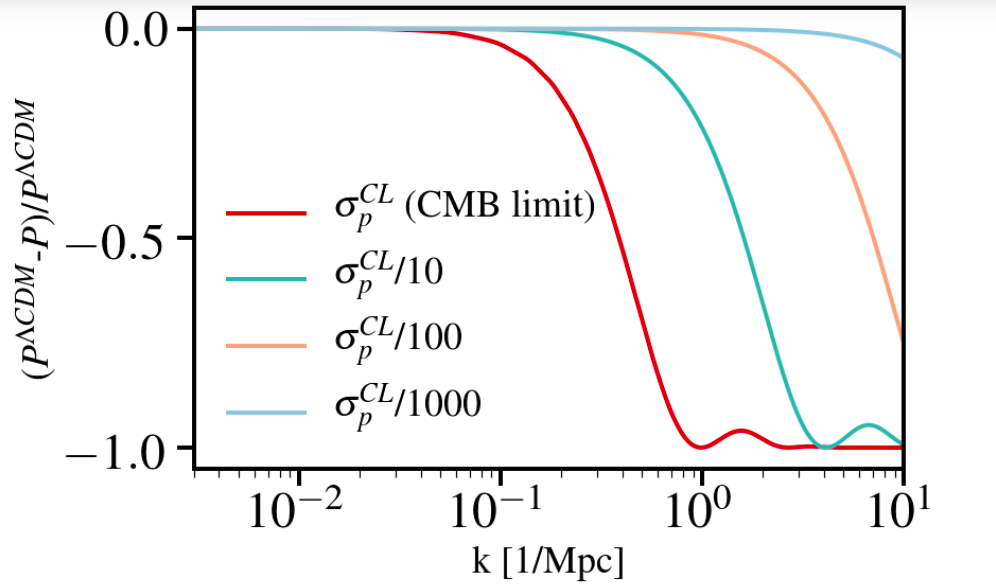
\includegraphics[width=0.6\columnwidth]{figures/dmbaryon_pk.png}
\caption{Linear matter power spectrum at $z=0$. We show the residuals between the CDM case and the case where there is velocity-independent spin-independent scattering between dark matter and protons. The dark matter particle mass is set to 1 MeV, and all other cosmological parameters are set to their best-fit Planck 2015 values \citep{Ade:2015xua}. Different residual curves display cutoffs at different angular scales, controlled by the magnitude of the interaction cross section. The highest cross section shown corresponds to the current 95\% confidence-level upper limit inferred from analyses of CMB data \citep{Gluscevic:2017ywp,Boddy:2018kfv}.
\ADW{I think we need a better version of this figure.}
}
\label{fig:dmbaryon_pk}
\end{figure}
As an example, a measurement of the minimum halo mass translates into an upper limit on the dark matter-proton interaction cross section, based on the corresponding cutoff in the matter power spectrum $P(k)$; Figure \ref{fig:dmbaryon_pk} shows how the position of the cutoff in the linear $P(k)$ varies as a function of the interaction cross section. For example, a lower limit on the cutoff of $k_\text{cutoff}\sim 10/$Mpc roughly corresponds to an upper limit on the cross section which is 100 times more stringent than the current limit from CMB searches. Using limits on WDM as a proxy for a suppressed $P(k)$, and the illustration in Figure \ref{fig:dmbaryon_pk} to guide the eye, a minimum halo mass of $10^8$ solar masses would imply more than three orders of magnitude improvement over the current best cosmological limits on the interaction cross section.

%\ADW{I've commented these out because I think it is more productive to focus on specific models.}
%{\it Weakly-Interacting Massive Particles (WIMPs)}: In the WIMP paradigm, the dark matter candidate has a mass of $\roughly 100 \GeV$ and interacts with Standard Model particles via weak-scale interactions. In the early universe, the WIMP can be produced in the thermal bath of Standard Model particles, and its abundance is set by the so-called “freeze-out” process, i.e., when the annihilation rate between two WIMPs to Standard Model particles drops below the Hubble expansion rate, the co-moving number density of WIMPs remains nearly constant over the evolution. It turns out the weak-scale interactions lead to a WIMP relic abundance, consistent with the observed dark matter abundance. Over the past thirty years, the WIMP paradigm has motivated a number of searches in terrestrial experiments, including dark matter direct and indirect experiments, as well as collider experiments. The WIMP is a typical CDM candidate, and for a WIMP mass of $\roughly 100 \GeV$ the minimal halo mass is $\roughly 1 M_\Earth$.

%{\it Asymmetric dark matter}: The asymmetry between baryons and anti-baryons is well-documented in the visible sector, and can be trivially generalized to the dark matter sector. In this theory, the dark matter abundance is set by some primordial asymmetry in the early universe and further annihilation deplete the asymmetry component and only dark matter presents in the present universe. An attractive feature of this theory is that both dark matter and baryonic matter can be co-generated in the early universe and it explains the observational coincidence that the dark matter abundance is 5 times higher than the baryon abundance. For asymmetric dark matter, the typical dark matter mass is close to $5~{\rm GeV}$, five times the proton mass. For asymmetric dark matter, indirect detection signals from dark matter annihilation are typically absent, while direct and collider signals would be similar as in the WIMP case.

%{\it Hidden sector dark matter}: given the fact that we have not seen any signals from the terrestrial searches, there has been growing interest in the hidden sector dark matter theory. It assumes the dark matter is just one component of a more complex dark sector that may compose of multiple particle species. In the early universe, these hidden particles can be produced through inflaton decays, similar to the standard model particles. The dark matter abundance can be set by the freeze-out or asymmetric mechanisms. In some realizations, one can still preserve the virtue of the WIMP miracle. The hidden sector could also couple to the standard model sector through some portals, e.g., kinetic mixing, Higgs and neutrino mixings. And these mixing portals may lead to indirect and direct detection signals. In addition, if these portal terms present, the dark matter abundance can be produced through the freeze-in mechanisms, or even the hidden sector can be thermalized with the standard model sector. However, since the correlation between the dark matter abundance and the mixing parameter is loosened, compared to the WIMP case, it is possible to have the correct relic abundance while being consistent with the terrestrial constraints. In the hidden dark matter theory, model constraints on the dark matter mass and interactions are typically weak, which allows large model parameters subject to astrophysical probes. Possibilities are richer compared to the WIMP case.
%\ADW{I think this needs to be connected back to LSST. For example, coupling between dark matter and dark radiation can be constrained via ETHOS-like frameworks.}
